\documentclass[a4paper,12pt]{article}
\usepackage[T1]{fontenc}
\usepackage{inputenc}
\usepackage{fontspec}
\usepackage{lmodern}
\usepackage[english]{babel}
\usepackage{hyperref}
\usepackage{float}
\usepackage{tikz} % pour la définition de couleur
\usepackage{soul} % pour surligner le texte

\usepackage[margin=2.3cm]{geometry} % marges

% MISE EN FORME DES BLOCS DE CODE
\usepackage{listings} % pour les blocs de code

\definecolor{whitegray}{gray}{0.97}
\definecolor{pearlgray}{gray}{0.94}
\definecolor{lightgray}{gray}{0.90}
\definecolor{darkgray}{gray}{0.50}
\definecolor{green}{rgb}{0.22, 0.73, 0.56}
\definecolor{red}{rgb}{0.8, 0.25, 0.33}
\definecolor{blue}{rgb}{0.36, 0.62, 0.92}
\definecolor{bluegray}{rgb}{0.33, 0.41, 0.47}

% Pour que le texte en police console soit surligné en gris clair
\let\OldTexttt\texttt
\sethlcolor{pearlgray}
\renewcommand{\texttt}[1]{\OldTexttt{\hl{#1}}}

% Pour la colorisation des nombres dans le code seulement quand il ne font pas partie de chaine de caractères ou commentaire
\newcommand\digitstyle{\color{blue}}
\makeatletter
\newcommand{\ProcessDigit}[1]
{%
	\ifnum\lst@mode=\lst@Pmode\relax%
	{\digitstyle #1}%
	\else
	#1%
	\fi
}

% Definition de l'apparence des blocs de code
\lstset{
	language=php, % définition du langage (php et javascript ont des syntaxes proches)
	basicstyle=\scriptsize\ttfamily, % petite taille, police de console
	stringstyle=\color{red}, % chaine de caractères
	backgroundcolor=\color{whitegray}, % fond
	commentstyle=\color{darkgray}\textit, % commentaires
	numberstyle=\tiny\color{darkgray}, % numero de ligne
	rulecolor=\color{lightgray}, % bordure
	keywordstyle=\color{green}\textbf, % opérateurs logiques etc
	literate=
	{0}{{{\ProcessDigit{0}}}}1
	{1}{{{\ProcessDigit{1}}}}1
	{2}{{{\ProcessDigit{2}}}}1
	{3}{{{\ProcessDigit{3}}}}1
	{4}{{{\ProcessDigit{4}}}}1
	{5}{{{\ProcessDigit{5}}}}1
	{6}{{{\ProcessDigit{6}}}}1
	{7}{{{\ProcessDigit{7}}}}1
	{8}{{{\ProcessDigit{8}}}}1
	{9}{{{\ProcessDigit{9}}}}1
	{<=}{{\(\leq\)}}1,
	morestring=[b]",
	morestring=[b]',
	morecomment=[l]//,
	aboveskip=3mm,
	belowskip=-2mm,
	breakatwhitespace=false,
	breaklines=true,
	captionpos=b,
	deletekeywords={...},
	escapeinside={\%*}{*)},
	extendedchars=true,
	framexleftmargin=16pt,
	framextopmargin=5pt,
	framexbottommargin=5pt,
	frame=tblr,
	keepspaces=true,
	morekeywords={*,...},
	numbers=left,
	numbersep=10pt,
	showspaces=false,
	showstringspaces=false,
	showtabs=false,
	stepnumber=1,
	tabsize=4,
	title=\lstname,
}

\begin{document}
\section{Features}\label{features}

The ``Segolene-front-office'' branch mostly concerns the historical part of the navigation in the front office. Several modules where developped~:
\begin{itemize}
	\item Data visualisations~;
	\item Sidebar for metadata~;
	\item Search interface~;
	\item Bread crumbs~;
	\item Related table editions.
\end{itemize}

NB : the presented functions are here often simplified for demonstration purposes comparing to the way they are integrated into the code.

\subsection{Data visualisation}\label{data-visualisation}

\subsubsection{Visualisation description}\label{visualisation-description}

Three different visualisations were developped for the historical navigation with the AmCharts library :
\begin{itemize}
	\item \textbf{Column chart} : visualisation for the work record page. Each column represents a primary source divided in original items (the cells) which colors are determined by their astronomical object~; the visualisation allows to show completeness and content of the sources derived from a intellectual work.
\end{itemize}

\begin{figure}[H]
	\centering
	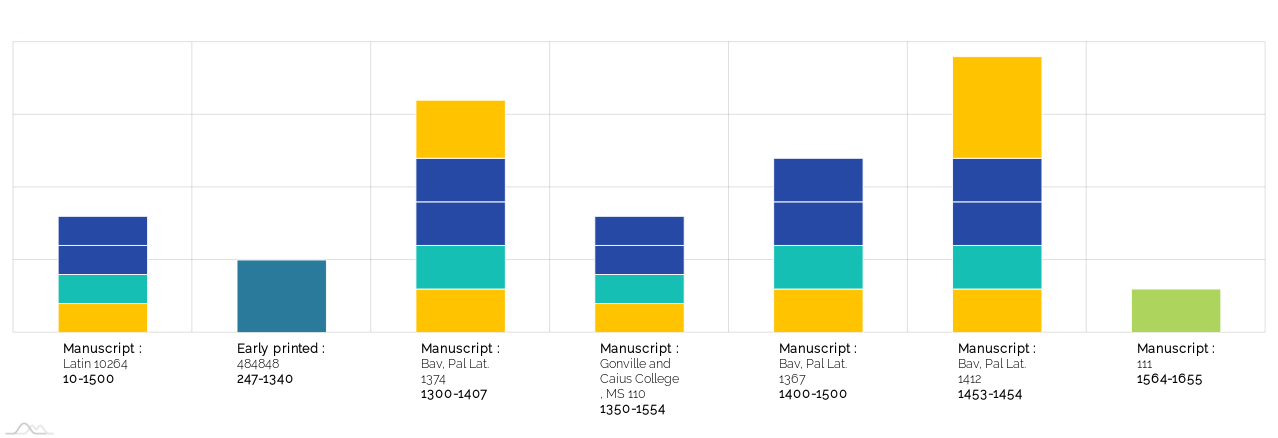
\includegraphics[width=16cm]{Images/Visualisations/Work-Tabule_Magne.png}
	\caption{Column chart for work visualisation}
\end{figure}

\begin{itemize}
	\item \textbf\textbf{Bar chart} : visualisation for the primary source record page. Each bar represents a work that is contained in the primary source, each bar being divided in original items originated from the work. A select allows two switch between two states of the visualisation : one where all pages of the items are added together, one where they are disposed accordingly to their position in the source. The visualisation thus can show the composite aspect of some primary sources.
\end{itemize}

\begin{figure}[H]
	\centering
	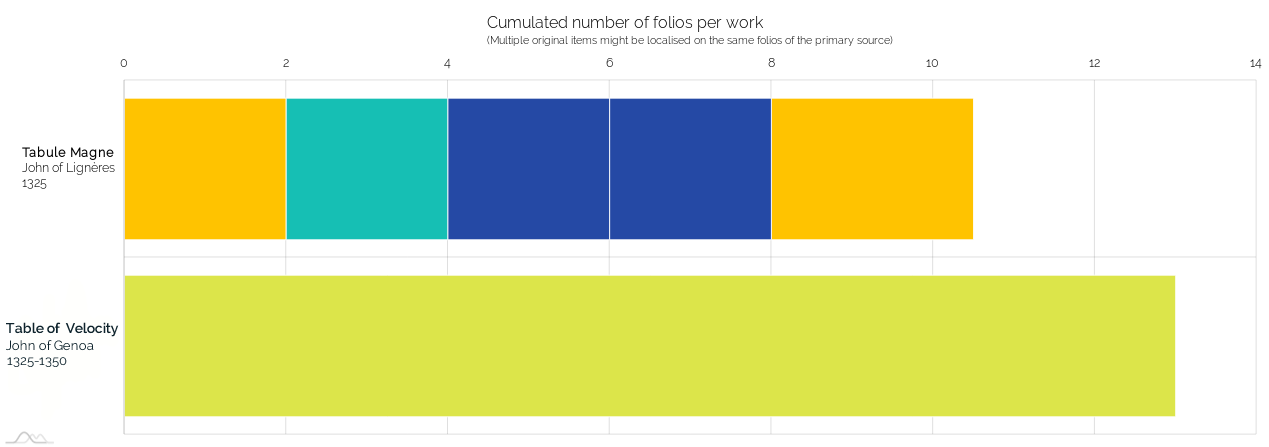
\includegraphics[width=16cm]{Images/Visualisations/Primary_source-Stacked.png}
	\caption{Bar chart for primary source visualisation~: original items stacked}
\end{figure}
\begin{figure}[H]
	\centering
	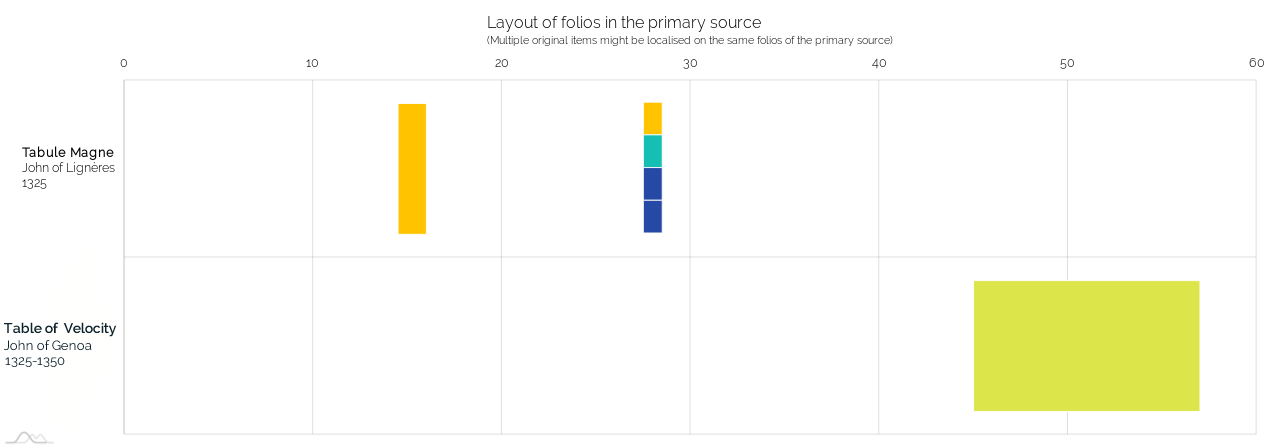
\includegraphics[width=16cm]{Images/Visualisations/Primary_source-Spread_out.png}
	\caption{Bar chart for primary source visualisation~: original items spread out}
\end{figure}

\begin{itemize}
	\item \textbf{Historical map} : visualisation for the original item records, the historical navigation and more to come. The map displays points that represent the place of creation of works (in yellow), primary sources/original items (in red) and combination of both (in orange). A heatmap underneath represents the time axis and show what period were more prolific : the scrollbar allows the user to select a time period so that only the items created during the timerange are shown.
\end{itemize}

\begin{figure}[H]
	\centering
	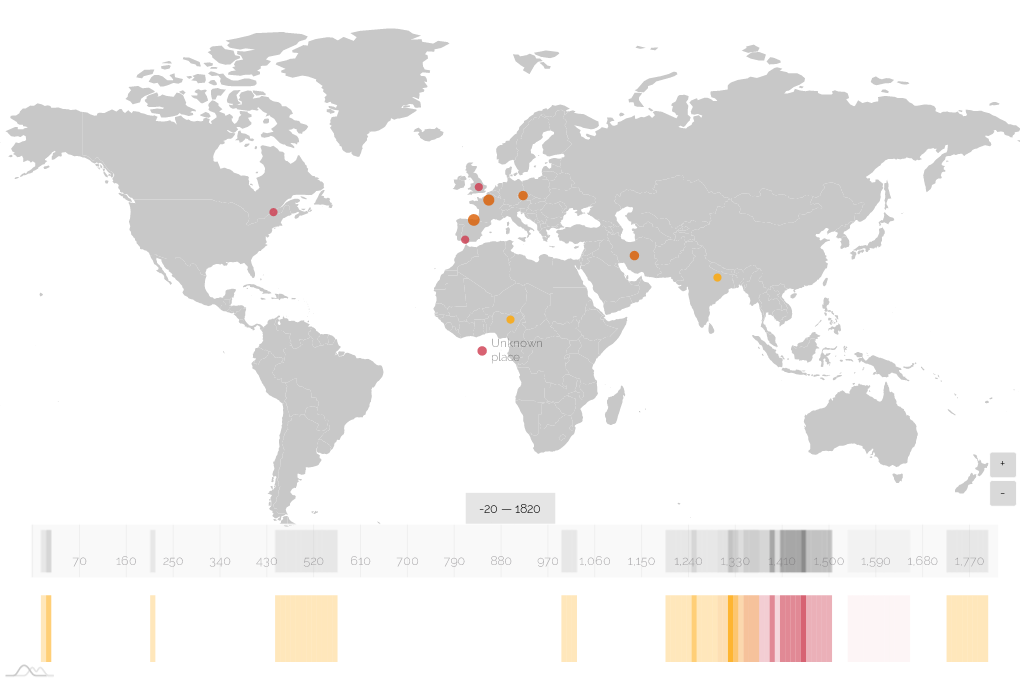
\includegraphics[width=16cm]{Images/Visualisations/Historical_navigation-All.png}
	\caption{Map for historical navigation}
\end{figure}

\subsubsection{Function explanation}\label{function-explanation}

\paragraph{Historical map}\label{historical-map}

This function is triggered when the user change the range selected by the scrollbar. What it does is that each time the start and the end grips of the scrollbar are both outside (by being under or above it) of the \texttt{tpq} and \texttt{tap} dates of an item, the item is not shown on the map. When the grips are not both outside, the size, color, tooltip of the map point are set accordingly to the items that were created in the timerange selected.

\begin{lstlisting}
scrollbarX.events.on("rangechanged", function () {
    let cursorMin = scrollbarX.range.start;
    let cursorMax = scrollbarX.range.end;

    // Conversion of the min and max range value into date
    let dateMinRange = parseInt((cursorMin / yearRange) + startBar);
    let dateMaxRange = parseInt((cursorMax / yearRange) + startBar);
    // Show the timerange selected
    scrollbarX.startGrip.tooltipText = `${dateMinRange}`;
    scrollbarX.endGrip.tooltipText = `${dateMaxRange}`;
    timeframeLabel.text = `${dateMinRange} — ${dateMaxRange}`;

    i = 0;
    // for each place in mapData
    for (let index in mapData) {
        // defining appearance of the circle localised on the place
        let place = mapData[index];
        let opacity = 0; // if no item is to be displayed, opacity to 0
        let countW = 0; // count of the number of works to be displayed : color and radius of the circle
        let countPS = 0; // count of the number of primary sources to be displayed : color and radius
        let number = 0;

        for (let j = place.items.length - 1; j >= 0; j--) {
            let dateMin = (place.items[j].from - startBar) * yearRange;
            let dateMax = (place.items[j].to - startBar) * yearRange;
            if (!((cursorMin > dateMax && cursorMax > dateMax) || (cursorMin < dateMin && cursorMax < dateMin)))
                // when the two cursors are not both outside of the time frame selected
                // either by being under or above it
            {
                number++;
                opacity = 0.8; // set the opacity in order to not be transparent
                if (place.items[j].entity === "work") {
                    countW += 1; // add one to the count of works
                } else {
                    countPS += 1;
                }
            }
        }

        let Wtootltip = countW !== 0 ? "[bold]Work[/]\n‣ " + countW + " record(s)" : "";
        let PStootltip = countPS !== 0 ? "[bold]Primary source[/]\n‣ " + countPS + " record(s)" : "";

        let tooltip = "[font-size:18px]" + place.place + "[/]\n" + Wtootltip + PStootltip;
        number = number !== 0 ? number * 100 : 100;

        placeMarker[i].fillOpacity = opacity;
        placeMarker[i].radius = Math.log(number);
        placeMarker[i].tooltipText = tooltip;
        i++;
    }
});
\end{lstlisting}

\paragraph{Bar chart}\label{bar-chart}

This function is triggered when the user selects one or another option. If the option is ``page disposition'', the height and displacement of the cell are determined in relation to the number of items in the same bound as theirs. In other words, the more items there are on the same pages, the thiner and the more deported from the center will be the cell representing one item.
 
\begin{lstlisting}
function selectView(select) {
    if (select === "spread") {
        chart.data = spreadOutSet; // make the chart use the "spread out" data set
        let numberOfWorks = Object.keys(worksBounds).length;
        let heightWork = 292/numberOfWorks; // height of the horizontal part dedicated to one work
        let heightBar = 225/numberOfWorks; // height of the bar in itself

        for (let work of Object.keys(worksBounds)){
            bounds = worksBounds[work];
            for (key of Object.keys(bounds)){
                i = 0;
                let bound = bounds[key];
                let numberOfOrigItems = bound.origItems.length;
                for (let id of bound.origItems) {
                    let heightItem = heightWork/numberOfOrigItems;
                    // setting the height of the cell
                    series[id].columns.template.height = heightItem;
                    // configuring the displacement of the cell comparing to the center
                    if (heightItem !== heightWork){
                        series[id].columns.template.dy = -(heightBar/2) + (heightItem * i);
                    }
                    i++;
                }
            }
        }
    } else if (select === "stack") {
        chart.data = stackedSet; // make the chart use the "stacked" data set
        for (id of ids){
            series[id].columns.template.dy = 0;
            series[id].columns.template.height = am4core.percent(80);
        }
    }
}
\end{lstlisting}

After creating an object detailling how the different items are disposed in the primary source (\texttt{workBounds = \{"workTitle1" :[\{bound : [min, max], origItems : [id1, id2]\},\{bound : [min, max], origItems : [id3]\}], "workTitle2" : [...]\}}), some items being on the same pages, each series of the chart (i.e.~each cell) is individually styled according to how the items are disposed.

\subsection{Sidebar of metadata}\label{sidebar-of-metadata}

The sidebar is a template that is integrated to the record pages of work, primary source and original item. The template is filled with an associative array filled with metadata of the record that is being displayed : this associative array is build thanks to the \texttt{getMetadataTable()} method located in each repository of the concerned entities.

\begin{figure}[H]
	\centering
	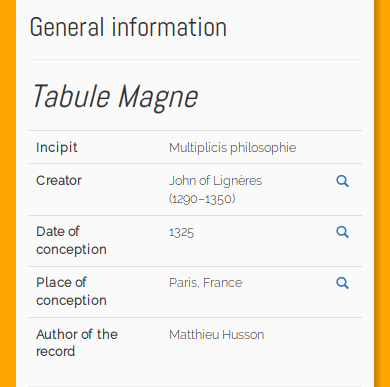
\includegraphics[width=10cm]{Images/Sidebar/metadata-work.png}
	\caption{Metadata display in the sidebar}
\end{figure}

\paragraph{Data struture}\label{data-struture}

The data produced by the \texttt{getMetadataTable()} method is always structured the same way in order to correctly generate the sidebar using the template \texttt{sideMetadata.html.twig}.

\begin{lstlisting}
$metadata = ["entity" => $entityName // index name that will be used to construct an Elastisearch query
         "title" => $title, // text to display in the upper part of the sidebar
        ("subtitle" => $subtitle), // facultative
         "field name" => ["values" => ["text to display"],
                  "search" => ["json" => ["query to send to ElasticSearch"],
                           "hover" => "text to display when hovering the magnifier"],
                       "title" => ["title of the query"]],
         "other field" => ["values" => [["html" => "text to display", // when text must be a link
                         "id" => "id of the entity for the link",
                         "path" => "path name to construct link"]],
                   "search" => ["json" => [],// no magnifier when this array is empty
                        "hover" => ""],
                        "title" => []]
];
\end{lstlisting}

Each key of the array (except for the key \texttt{entity}) corresponds to a field that is going to appear in the sidebar. The upper part of the sidebar is filled with the keys \texttt{"title"} and \texttt{"subtitle"} (not required), and for the part in the white insert, each key constitutes the text that is going to appear as field name.

To each of these keys is attached an associative array defining how the metadata related to these fields are going to be displayed. Each key referes to something specific :
\begin{itemize}
	\item  \textbf{values} : the text in \texttt{html} that is going to appear next to the field name. In the array associated to this key, can be added an array if the text is going to be a link~:
	\begin{itemize}
		\item \textbf{html} : text to display
		\item \textbf{id} : id of the entity in order to build the link
		\item \textbf{path} : path of the page to redirect to 
	\end{itemize}
	\item \textbf{search} : data used for generating the magnifier (i.e.~redirecting to the search page for more related items). To this key is attached an other associative array~:
	\begin{itemize}
		\item \textbf{json} : query in the DSL language of ElasticSearch. Not all the query is needed, only the \texttt{query} part. The \texttt{source}, \texttt{size}, etc are generated after that.
		\item \textbf{hover} : text that is going to appear when hovering the magnifier, which is a description of the query
		\item \textbf{title} : title of the query that will appear in the result page
	\end{itemize}
\end{itemize}

The keys \texttt{values}, \texttt{json} and \texttt{title} are associated to an array because some fields can have several values to display, for instance is a work has multiple creators. For example, if a primary source is written in two different scripts, the metadata associated to the ``script field'' will look like this~:

\begin{lstlisting}
["scripts" =>
   ["values" =>
       ["<span class='mainContent'>Latin</span>",
        "<span class='mainContent'>Gothic</span>"],
    "search" =>
       ["json" =>
           ['["bool":["must"=>[[["match"=>["original_texts.script.id"=>85}}]]}}',
            '["bool":["must"=>[[["match"=>["original_texts.script.id"=>46}}]]}}'],
        "hover" =>"Find all primary sources written in the same script",
        "title" => 
           ["All primary sources written in latin",
            "All primary sources written in gothic"]
     ]
 ];
\end{lstlisting}

\paragraph{String formatting}\label{string-formatting}

The text that is going to be displayed is formatted thanks to the \texttt{toPublicString} and \texttt{toPublicTitle} methods~:
\begin{itemize}
	\item  \texttt{toPublicString} is used when the information will be displayed as metadata (i.e.~in the record page of an original item, the name of the work of this item will be formatted with this method)~;
	\item \texttt{toPublicTitle} is used when the information will be displayed as main content (i.e.~in the record page of a work, the name of the work will be formatted with this method).
\end{itemize}

The \texttt{getTpaq()} methods returns for each entity associated with a tpq and a taq date, a correctly formatted date, for example :
\begin{itemize}
	\item if \texttt{tpq} = 1245, and \texttt{taq} = 1325 ==\textgreater{} ``1245---1325''
	\item if \texttt{tpq} = 1325, and \texttt{taq} = 1325 ==\textgreater{} ``1325''
\end{itemize}

\paragraph{Managing missing information}\label{managing-missing-information}

If an information is missing, (for example, if the current entity doesn't have place associated with it), several layout options are available :
\begin{itemize}
	\item textbf{\emph{Not showing the field at all}} : the key for this field must not appear in the array of metadata, or the array associated to the \texttt{values} key must be lefted empty.
\end{itemize}

\begin{lstlisting}
// the field translator must appear only if there is one
if ($work->getTranslator()){
    $metadata["translator"] = $metadataTable;
    $metadata["translator"]["values"][] = $work->getTranslator()->toPublicString();
}
\end{lstlisting}

\begin{itemize}
	\item \textbf{\emph{Showing the field with a string indicating the missing information}} : in the array associated to the \texttt{values} key, a string can be set when there is no information available for the current field. It must be encapsulated in a \texttt{\textless{}span class="noInfo"\textgreater{}\textless{}/span\textgreater{}} tag.
\end{itemize}

\begin{lstlisting}
// if there is no incipit, display "Missing incipit"
$incipit = $work->getIncipit() ? $work->getIncipit() : "<span class='noInfo'>Missing incipit</span>";
\end{lstlisting}

\begin{itemize}
	\item \textbf{\emph{Keeping the field empty of information}} : when the array of the \texttt{values} key is lefted with an empty string in it, the template of the sidebar will automatically display \texttt{\textless{}span class="noInfo"\textgreater{}No information provided\textless{}/span\textgreater{}}
\end{itemize}

\begin{lstlisting}
// if there is no historical actors, set the values to be [""]
$values = count($actors) != 0 ? [] : [""];
\end{lstlisting}


\paragraph{Pie chart}\label{pie-chart}

A pie chart can be displayed a the bottom of the sidebar when creating a key named \texttt{visualisation} in the metadata array, filled with an associative array defining a title and a dataset for the chart.

\begin{lstlisting}
$metadata["visualization"] = [
    "title" => "Title of the visualisation"
    "data" => [["category" => "cat1", "value" => 7],["category" => "cat2", "value" => 4],[...]]
];
\end{lstlisting}

\begin{figure}[H]
	\centering
	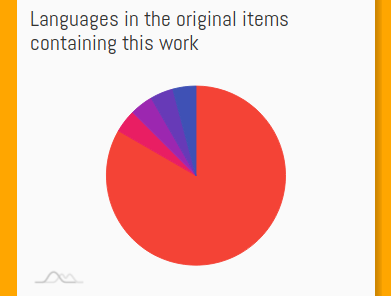
\includegraphics[width=10cm]{Images/Sidebar/pie-work.png}
	\caption{Pie chart at the bottom of the sidebar}
\end{figure}

\subsubsection{Sidebar template}\label{sidebar-template}

The sidebar is opened with a click on a toolbar icon, and closed when clicked outside the sidebar. The javascript allows to switch between two states that are defined in the public CSS stylesheet : when opened, the classes \texttt{open-toolbar} and \texttt{open-sidebar} are added to the element of the sidebar in order to appear on the page.

\begin{lstlisting}
$(document).ready(function(){
    // open the sidebar on a toolbar item
    $('.toolbarItem>span').click(function(){
        let id = $(this).attr('id');

        $("#sidebar").attr("isOpen", "true");
        switchSidebar();
        let sideContent = "side-"+id;
        $('.backgroundSidebar').hide();
        $('#'+sideContent).show();
    });

    // close the sidebar when clicked outside the side bar
    $(document).click(function (e) {
        let thatTarget = $(event.target);
        // if the clicked target is not a child of sidebar AND sidebar is open
        if (!thatTarget.closest('#sidebar').length && $("#sidebar").attr('isOpen') === "true"){
            $("#sidebar").attr("isOpen", "false");
            switchSidebar();
        }
    });

    function switchSidebar() {
        if ($("#sidebar").attr("isOpen") === "false") {
            $("#sideBorder, #toolbar").removeClass("open-toolbar");
            $("#innerSidebar").removeClass("open-sidebar");
        } else {
            $("#sideBorder, #toolbar").addClass("open-toolbar");
            $("#innerSidebar").addClass("open-sidebar");
        }
    }
});
\end{lstlisting}

\subsection{Search interface}\label{search-interface}

The search page serves for now two purposes~:
\begin{itemize}
	\item allowing the user to perform full-text queries, only on the entities \textbf{work}, \textbf{primary source} and \textbf{original item},
	\item displaying the related items when clicking on a magnifier in the sidebar of a entity record.
\end{itemize}

The queries are performed on the ElasticSearch database through an AJAX call : TODO when launching in production, the requested server (from \texttt{localhost} to \texttt{dishas.obspm}) will change. The variable to be modified to make this change is located in the \texttt{myElasticSearch.js}~:

\begin{lstlisting}
function generateUrl(query="", index="", from = 0, size = 10000, server="localhost:9200", http="http") { ... }
\end{lstlisting}

The retrieved results from this call are then formatted to be displayed in a DataTable thanks to the \texttt{TAMASListTableTemplate} objects. Those templated are defined with the \texttt{getPublicObjectList()} in the entity repositories.

\subsubsection{Data structure : \texttt{TAMASListTableTemplate}}\label{data-structure-tamaslisttabletemplate}

The templates defines for each field (i.e.~column) of an entity how the information is going to be presented inside the DataTable. For instance, the template of a work title will defined that the text is going to be in \emph{italic}, \href{}{redirect} to the page of the concerned work and that the string ``Unknown title'' will be displayed if the information is missing.

The \texttt{getPublicObjectList()} is defined as follows :

\begin{lstlisting}
public function getPublicObjectList()
    {
        $fieldList = [
            new TAMASListTableTemplate(
                'name of the key where the information in the array of result will be located',
                'Column title for this field',
               ['class'=>['array of CSS classes to style the text'],
                'path' => 'defined if a the text is a link',
                'id' => 'name of the key where the id in the results is located'],
                'unknown' => 'text to display if the information is missing',
                'fields needed to display this field, correspond to the `_sources` in a ElasticSearch query'
        )];

        return $fieldList;
    }
\end{lstlisting}

Each column needs its template, each entity combining between 5 and 10 templates. A template object can be defined with a certain number of properties~:

\begin{itemize}
	\item \textbf{Name}~: provides the location in an array where DataTable will find the information to display
	\item \textbf{Title}~: corresponds to the column label associated with the information
	\item \textbf{Properties}~: defines how the cell content will be formatted~:
	\begin{itemize}
		\item \textbf{class} (will surround the text in a \texttt{\textless{}span class="\_\_"\textgreater{}\textless{}/span\textgreater{}})~:
		\begin{itemize}
			\item \textbf{\emph{list}} : to indicate that multiple values can be displayed in the same cell
			\item \textbf{\emph{number}} : in order to align the text to the right
			\item \textbf{\emph{title-italic}} : to style the text of the cell in italic
		\end{itemize}
		\item \textbf{path} + \textbf{id}~:
		\begin{itemize}
			\item \textbf{\emph{path}} : routing path to generate a link
			\item \textbf{\emph{id}} : location of the id in the result object
		\end{itemize}
	\end{itemize}
	\item \textbf{Source} : defines which fields will appear in the elasticsearch response corresponding to the fields that are added to the array associated with the key ``source'' in the query (multiple fields can be added for a single column with ``+'')
\end{itemize}

\begin{lstlisting}
// Field "Work" of an original item defining how the work titles will appear
new TAMASListTableTemplate(
    'work',
    'Work',
    ['class' => ['title-italic'], 'path' => 'tamas_astro_viewWork', 'id' => 'work.id'],
    '', // ifOnly is not used in the public interface
    'work.default_title+work.id'
)
\end{lstlisting}

\subsubsection{Specific functions}\label{specific-functions}

The functions and variables used to create the search interface are located in several files~:
\begin{itemize}
	\item \texttt{publicResult.html.twig} : twig template for the result page
	\item \texttt{myElasticSearch.js} : functions to build queries, to retrieve data from response or generate URL
	\item \texttt{myDataTable.js} : functions related to DataTables
	\item \texttt{mainJavascript} : utility functions
\end{itemize}

The main functions help :
\begin{itemize}
	\item to \textbf{retrieve results} from ElasticSearch
\end{itemize}

\begin{lstlisting}
/**
* This function takes a response from an ajax call to elasticsearch
* and returns an array containing all the results of this query
*
* @param queryResponse : object
* @return {Array}
*/
function retrieveResults(queryResponse) {
    if (typeof queryResponse.hits.hits !== 'undefined') {
        let data = queryResponse.hits.hits; // data is an array of results, but only the value of the key "_source" is needed
        let results = [];

        $.each(data, function (key, value) {
            results.push(value._source);
        });

        return results;
    }
}
\end{lstlisting}

\begin{itemize}
	\item to \textbf{format those results} (using the properties defined in the \texttt{TAMASListTableTemplate})
\end{itemize}

\begin{lstlisting}
/**
* to either return the information associated with a field
* or return a tag indicating missing information
* The properties will defined how the cell content is formatted.
*
* @param text : result values to display inside an array (even if there is only 1 value)
* @param properties : object defined in the template object list (getPublicObjectList)
* @param result : object containing the results send by Elasticsearch
* @returns string
*/
function textDisplay (text, properties=[], result={}){
    let classes = "";
    if (isDefined(properties.class)){ // putting all classes in the same string
        for (let i = 0; i < properties.class.length; i++){
            let className = properties.class[i];
            classes = classes + className;
            classes = i < properties.class.length ? classes + " " : "";
        }
    }

    if (isDefined(text)){
        if (isDefined(properties.path)){
            let id = [selectNodeOfObject(properties.id, result)];
            // selectNodeOfObject will select the id in the result if there is only one id to find,
            // unlike when the cell is supposed to contain a list
            if (isDefined(properties.class) && properties.class.includes("list")){
                // if the cell is supposed to contain a list of links
                // the "text" array looks like : ["text, id, "text", id, ...]
                let texts = [];
                id = [];
                for (let j = 0; j < text.length; j += 2){
                    texts.push(text[j]);
                    id.push(text[j+1]);
                }
                text = texts; // now it looks like ["text","text", ...]
            }
            let linkText = [];
            for (i = 0; i < text.length; i++){
                linkText.push(`<a href="${generateRoute(properties.path, id[i])}">${text[i]}</a>`);
            }
            text = linkText;
        }

        let cellContent = "";
        let cellSummary = "";
        for (i = 0; i < text.length; i++){
            if (i === 0){
                cellContent = classes !== "" ? `<span class="${classes}">${text[i]}</span>` : `${text[i]}`;
            } else {
                cellSummary = cellSummary + `<span class="${classes}">${text[i]}</span>`;
                cellSummary = i < text.length ? cellSummary + "<br/>" : "";
            }
        }
        if (text.length > 1){ // if there is multiple data to display, put it in a summary
            let Nrecord = text.length > 2 ? "s" : "";
            let summary = `<summary class="mainContent">
                                        ${text.length-1} <span style="font-variant: small-caps">more record${Nrecord} </span>
                                        <span style="font-size: 10px">▼</span>
                                    </summary>`;
            cellContent = `${cellContent}<details>${summary}${cellSummary}</details>`;
        }
        return cellContent;
    } else { // if the key doesn't exist in the array of results => missing information
        if (isDefined(properties.unknown)){
            return `<span class='noInfo'>${properties.unknown}</span>`;
        }
        return "<span class='noInfo'>No information provided</span>";
    }
}
\end{lstlisting}

\begin{itemize}
	\item to \textbf{display those results} in a \texttt{DataTable}
\end{itemize}

\begin{lstlisting}
/**
* This function generates an entire Datatable of results retrieved from a query to elasticsearch
* on the given index for the filters given as parameter query
*
* it generates by default a query of a size 10000, from 0
*
* @param index string : label of an entity (ex : "primary_source")
* @param query object : the filters of the query (ex: {"match":{"id":"5"}})
*                      => the value associated with the key "query" in the query language of elasticsearch
* @param queryTitle string : title detailing the query in natural language (EX => "All original items kept in the British Library")
* @param queryTerm string : terms used to filter the results
* @param from int : the number of results from which the query starts
* @param size int : number of results wanted in the response
* @param generateHeader bool : defines if the header is generated or not
* @return url : url of the query
*/
function generateResultTable(index, query, queryTitle="", queryTerm="", from=0, size=10000, generateHeader=true) {
    let fieldList = fieldLists[index];
    let dataStructure = generateDataStructure(fieldList);
    let sourceFields = generateSources(fieldList, true);

    // generates columns labels
    generateColumnHeader("results", fieldList)

    // generates URL in order to make an ajax call
    let url = generateUrl(query, index, from, size);

    // defining the function formatting the response of an elasticsearch ajax call
    // into an array of results ready to be displayed by DataTable
    let formatData = function (queryResponse){
        let results = retrieveResults(queryResponse);
        for (let result of results){
            let i = 0;
            for (let field of fieldList){
                // field.name is the key where DataTable is going to search for the value to fill the cells of one specific column
                // textDisplay() returns the value that is going to be displayed in the cell :
                // 		- the text correctly formatted (according to the field.properties)
                // 		- OR no information provided (if there is no value in the result array)
                // selectNodeOfObject() returns the value of the node in the array of result
                // corresponding to string given as first argument
                result[field.name] = textDisplay(selectNodeOfObject(sourceFields[i], result, field.properties), field.properties, result);
                i++;
            }
        }
        return results;
    };

    if (generateHeader){
        // generates a header for the current query
        generateSearchHeader(index, queryTitle, queryTerm);
    }

    let table = $('#results').DataTable({
        "ajax": {
            "url": url, // url on which the query is done
            cache: true, // mandatory in order to send the query without wildly added parameters
            "dataSrc": formatData // variable containing the function formatting the results in order to fill the DataTable
        },
        "columns": dataStructure, // specify where DataTable will find information associated with each fields
        });
    return url;
}
\end{lstlisting}

\subsection{Bread crumbs and table editions}\label{bread-crumbs-and-table-editions}

\subsubsection{Bread crumbs}\label{bread-crumbs}

The breadcrumbs allows the user to find his way around the front office, it indicates at which level of the site hierarchy they are located. The javascript code to generate them takes as argument the name of the current node, i.e.~the name of the page, and it reconstructs the page tree structure to get there.

\begin{lstlisting}
// define an array to contain the dependance tree of the current page
let nodeTree = [];
nodeTree.push(currentNode);
let node = currentNode;

for (nav of nodeTree){
    if (navigation[nav]){ // navigation contains all the nodes associated with their parent node
        nodeTree.push(navigation[nav]);
    }
}

if (!(nodeTree.length <= 1)){
    // reverse the order of the array to put the greater parent first
    nodeTree.reverse();

    // create a breadcrumb for each node of the nodeTree object
    for (let l = 0; l < nodeTree.length ; l++){
        node = nodeTree[l];
        // set the pictogram image of the current node
        let picto = "{{ asset('img/pictograms/'~'INTERFACENAME'~'.png') }}";
        picto = picto.replace("INTERFACENAME", node);

        if (properties[node]["path"] !== ""){
            // generate a route for the current node
            let route = Routing.generate(properties[node]["path"]);
        }

        $(".breadcrumb-icons").append(`<div class="col-md-1 picto-bundle">
                                        <a href="${route}" title="${properties[node]["hover"]}">
                                            <div class="picto-background ${currentNode}">
                                                <img class="picto-size"
                                                     src="${picto}"
                                                     alt="${properties[node]["title"]} pictogram">
                                            </div>
                                        </a>
                                    </div>
                                    <div class="col-md-1 chevron">
                                        <span class="glyphicon glyphicon-chevron-right"></span>
                                    </div>`);
    }
}
\end{lstlisting}

\subsubsection{Related table editions}\label{related-table-editions}

The relation of the edited texts and the original texts are modelled in a graph structure in order to limit aberration and loops (preventing an edition to be based on an edition that is itself based upon this edition), and to display graph visualisations for the editions. With the aim of gathering all the editions that were based on one particular original item, including the \emph{indirect} ones (type B editions), it is necessary to use the graph structure.

\texttt{DISHAS/src/TAMAS/AstroBundle/Repository/OriginalTextRepository.php}

\begin{lstlisting}
/**
* getAllEditedTexts
*
* this method returns an array of the editions of an original item, including indirect editions (type B)
* 
* @param \TAMAS\AstroBundle\Entity\OriginalText $originalText
* @return array
*/
public function getAllEditedTexts(\TAMAS\AstroBundle\Entity\OriginalText $originalText)
{
   if (! $originalText)
      return [];

   $editedTextRepo = $this->getEntityManager()
      ->getRepository(\TAMAS\AstroBundle\Entity\EditedText::class);

   $dependanceTree = $editedTextRepo->getDependanceTree();
   $graph = new \TAMAS\AstroBundle\DISHASToolbox\Graph\TAMASGraph();
   $graph->loadJSONTree($dependanceTree);

   $origItemId = $originalText->getId();

   $originalId = 'o' . $origItemId; // the id of the original item is preceded by "o" in the graph tree
   $original = $graph->getNode($originalId); // find the node corresponding
   $editedTexts = $original->getAncestors(); // find the edited texts related to this node

   $editions = [];
   foreach ($editedTexts as $editedText){
      // fill the array with all the edited texts corresponding to the id
      $editions[] = $editedTextRepo->findBy(['id' => str_replace("e", "", $editedText->getLabel())])[0];
   }

   return $editions;
}
\end{lstlisting}

\end{document}
